\RequirePackage[table]{xcolor}
\documentclass[fonts]{icst}

\usepackage{moreverb}

\usepackage[breaklinks,colorlinks,bookmarksopen,bookmarksnumbered,linkcolor=ICSTblue,citecolor=blue,urlcolor=ICSTblue]{hyperref}
\usepackage{iftex}
\ifPDFTeX\usepackage{breakurl}\fi
\usepackage{doi}
\usepackage{xurl}

\usepackage[utf8]{inputenc}
\usepackage[english]{babel}
\usepackage{amsmath,amssymb,amsthm}
\usepackage{graphicx,flushend}
\usepackage{booktabs}
\usepackage{array}
\usepackage{multirow}
\usepackage{float}
\usepackage{enumitem}
\usepackage{dblfloatfix}
\usepackage{cuted}
\usepackage[hypcap=false]{caption}
\usepackage{adjustbox}
\usepackage{balance}
\usepackage{pifont}

% ---------------------------------------------------------------- revision helpers
% \pending{...} marks text whose final wording depends on runs still in progress.
% build.sh with FINAL=1 sets \pendingfalse; any remaining \pending is then an error.
\newif\ifpending\pendingtrue
\newcommand{\pending}[1]{\ifpending\textcolor{red}{[#1]}\else\errmessage{pending text left: #1}\fi}
\IfFileExists{generated/numbers.tex}{% generated by tools/paper_assets.py -- do not edit
\newcommand{\AvgDBal}{0.911}
\newcommand{\StdDBal}{0.000}
\newcommand{\NDBal}{1}
\newcommand{\AvgMBal}{0.954}
\newcommand{\StdMBal}{0.000}
\newcommand{\NMBal}{1}
\newcommand{\AvgFFBal}{0.993}
\newcommand{\StdFFBal}{0.000}
\newcommand{\NFFBal}{1}
\newcommand{\AvgDBiasGate}{0.920}
\newcommand{\StdDBiasGate}{0.000}
\newcommand{\NDBiasGate}{1}
\newcommand{\AvgMBiasGate}{0.958}
\newcommand{\StdMBiasGate}{0.000}
\newcommand{\NMBiasGate}{1}
\newcommand{\AvgFFBiasGate}{0.988}
\newcommand{\StdFFBiasGate}{0.000}
\newcommand{\NFFBiasGate}{1}
\newcommand{\AvgDBiasShift}{0.915}
\newcommand{\StdDBiasShift}{0.000}
\newcommand{\NDBiasShift}{1}
\newcommand{\AvgMBiasShift}{0.960}
\newcommand{\StdMBiasShift}{0.000}
\newcommand{\NMBiasShift}{1}
\newcommand{\AvgFFBiasShift}{0.993}
\newcommand{\StdFFBiasShift}{0.000}
\newcommand{\NFFBiasShift}{1}
\newcommand{\AvgDBiasln}{0.923}
\newcommand{\StdDBiasln}{0.009}
\newcommand{\NDBiasln}{2}
\newcommand{\AvgMBiasln}{0.958}
\newcommand{\StdMBiasln}{0.007}
\newcommand{\NMBiasln}{2}
\newcommand{\AvgFFBiasln}{0.995}
\newcommand{\StdFFBiasln}{0.001}
\newcommand{\NFFBiasln}{2}
\newcommand{\AvgDBiaslnAsy}{0.911}
\newcommand{\StdDBiaslnAsy}{0.000}
\newcommand{\NDBiaslnAsy}{1}
\newcommand{\AvgMBiaslnAsy}{0.970}
\newcommand{\StdMBiaslnAsy}{0.000}
\newcommand{\NMBiaslnAsy}{1}
\newcommand{\AvgFFBiaslnAsy}{0.994}
\newcommand{\StdFFBiaslnAsy}{0.000}
\newcommand{\NFFBiaslnAsy}{1}
\newcommand{\AvgDBitfit}{0.915}
\newcommand{\StdDBitfit}{0.000}
\newcommand{\NDBitfit}{1}
\newcommand{\AvgMBitfit}{0.959}
\newcommand{\StdMBitfit}{0.000}
\newcommand{\NMBitfit}{1}
\newcommand{\AvgFFBitfit}{0.995}
\newcommand{\StdFFBitfit}{0.000}
\newcommand{\NFFBitfit}{1}
\newcommand{\AvgDBitfitLC}{0.915}
\newcommand{\StdDBitfitLC}{0.000}
\newcommand{\NDBitfitLC}{1}
\newcommand{\AvgMBitfitLC}{0.959}
\newcommand{\StdMBitfitLC}{0.000}
\newcommand{\NMBitfitLC}{1}
\newcommand{\AvgFFBitfitLC}{0.995}
\newcommand{\StdFFBitfitLC}{0.000}
\newcommand{\NFFBitfitLC}{1}
\newcommand{\AvgDEffort}{0.912}
\newcommand{\StdDEffort}{0.001}
\newcommand{\NDEffort}{2}
\newcommand{\AvgMEffort}{0.960}
\newcommand{\StdMEffort}{0.008}
\newcommand{\NMEffort}{2}
\newcommand{\AvgFFEffort}{0.991}
\newcommand{\StdFFEffort}{0.001}
\newcommand{\NFFEffort}{2}
\newcommand{\AvgDGend}{0.923}
\newcommand{\StdDGend}{0.003}
\newcommand{\NDGend}{2}
\newcommand{\AvgMGend}{0.964}
\newcommand{\StdMGend}{0.003}
\newcommand{\NMGend}{2}
\newcommand{\AvgFFGend}{0.986}
\newcommand{\StdFFGend}{0.001}
\newcommand{\NFFGend}{2}
\newcommand{\AvgDLnBeta}{0.914}
\newcommand{\StdDLnBeta}{0.000}
\newcommand{\NDLnBeta}{1}
\newcommand{\AvgMLnBeta}{0.958}
\newcommand{\StdMLnBeta}{0.000}
\newcommand{\NMLnBeta}{1}
\newcommand{\AvgFFLnBeta}{0.985}
\newcommand{\StdFFLnBeta}{0.000}
\newcommand{\NFFLnBeta}{1}
\newcommand{\AvgDLnGamma}{0.914}
\newcommand{\StdDLnGamma}{0.000}
\newcommand{\NDLnGamma}{1}
\newcommand{\AvgMLnGamma}{0.961}
\newcommand{\StdMLnGamma}{0.000}
\newcommand{\NMLnGamma}{1}
\newcommand{\AvgFFLnGamma}{0.984}
\newcommand{\StdFFLnGamma}{0.000}
\newcommand{\NFFLnGamma}{1}
\newcommand{\AvgDLnLC}{0.921}
\newcommand{\StdDLnLC}{0.000}
\newcommand{\NDLnLC}{1}
\newcommand{\AvgMLnLC}{0.959}
\newcommand{\StdMLnLC}{0.000}
\newcommand{\NMLnLC}{1}
\newcommand{\AvgFFLnLC}{0.987}
\newcommand{\StdFFLnLC}{0.000}
\newcommand{\NFFLnLC}{1}
\newcommand{\AvgDProto}{0.907}
\newcommand{\StdDProto}{0.000}
\newcommand{\NDProto}{1}
\newcommand{\AvgMProto}{0.958}
\newcommand{\StdMProto}{0.000}
\newcommand{\NMProto}{1}
\newcommand{\AvgFFProto}{0.991}
\newcommand{\StdFFProto}{0.000}
\newcommand{\NFFProto}{1}
\newcommand{\AvgDRaAll}{0.921}
\newcommand{\StdDRaAll}{0.000}
\newcommand{\NDRaAll}{1}
\newcommand{\AvgMRaAll}{0.961}
\newcommand{\StdMRaAll}{0.000}
\newcommand{\NMRaAll}{1}
\newcommand{\AvgFFRaAll}{0.992}
\newcommand{\StdFFRaAll}{0.000}
\newcommand{\NFFRaAll}{1}
\newcommand{\AvgDRaFake}{0.923}
\newcommand{\StdDRaFake}{0.000}
\newcommand{\NDRaFake}{1}
\newcommand{\AvgMRaFake}{0.962}
\newcommand{\StdMRaFake}{0.000}
\newcommand{\NMRaFake}{1}
\newcommand{\AvgFFRaFake}{0.992}
\newcommand{\StdFFRaFake}{0.000}
\newcommand{\NFFRaFake}{1}
\newcommand{\AvgDRaGate}{0.917}
\newcommand{\StdDRaGate}{0.000}
\newcommand{\NDRaGate}{1}
\newcommand{\AvgMRaGate}{0.953}
\newcommand{\StdMRaGate}{0.000}
\newcommand{\NMRaGate}{1}
\newcommand{\AvgFFRaGate}{0.986}
\newcommand{\StdFFRaGate}{0.000}
\newcommand{\NFFRaGate}{1}
\newcommand{\AvgDRaProto}{0.918}
\newcommand{\StdDRaProto}{0.000}
\newcommand{\NDRaProto}{1}
\newcommand{\AvgMRaProto}{0.960}
\newcommand{\StdMRaProto}{0.000}
\newcommand{\NMRaProto}{1}
\newcommand{\AvgFFRaProto}{0.993}
\newcommand{\StdFFRaProto}{0.000}
\newcommand{\NFFRaProto}{1}
\newcommand{\AvgDRaReal}{0.929}
\newcommand{\StdDRaReal}{0.000}
\newcommand{\NDRaReal}{1}
\newcommand{\AvgMRaReal}{0.962}
\newcommand{\StdMRaReal}{0.000}
\newcommand{\NMRaReal}{1}
\newcommand{\AvgFFRaReal}{0.991}
\newcommand{\StdFFRaReal}{0.000}
\newcommand{\NFFRaReal}{1}
\newcommand{\AvgDRaRealLAD}{0.922}
\newcommand{\StdDRaRealLAD}{0.000}
\newcommand{\NDRaRealLAD}{1}
\newcommand{\AvgMRaRealLAD}{0.968}
\newcommand{\StdMRaRealLAD}{0.000}
\newcommand{\NMRaRealLAD}{1}
\newcommand{\AvgFFRaRealLAD}{0.993}
\newcommand{\StdFFRaRealLAD}{0.000}
\newcommand{\NFFRaRealLAD}{1}
\newcommand{\AvgDRaRealLD}{0.913}
\newcommand{\StdDRaRealLD}{0.000}
\newcommand{\NDRaRealLD}{1}
\newcommand{\AvgMRaRealLD}{0.936}
\newcommand{\StdMRaRealLD}{0.000}
\newcommand{\NMRaRealLD}{1}
\newcommand{\AvgFFRaRealLD}{0.982}
\newcommand{\StdFFRaRealLD}{0.000}
\newcommand{\NFFRaRealLD}{1}
}{}
\IfFileExists{generated/drift_numbers.tex}{% generated by tools/feature_figs.py -- do not edit
\newcommand{\DriftRealBitfit}{0.10}
\newcommand{\DriftFakeBitfit}{0.19}
\newcommand{\DriftRealRaReal}{0.98}
\newcommand{\DriftFakeRaReal}{0.93}
\newcommand{\DriftRealBiasln}{0.09}
\newcommand{\DriftFakeBiasln}{0.16}
\newcommand{\DriftRealGend}{0.47}
\newcommand{\DriftFakeGend}{0.37}
}{}
\newcommand{\num}[1]{\ifcsname #1\endcsname\csname #1\endcsname\else\textcolor{red}{??}\fi}
\newtheorem{proposition}{Proposition}

\newcommand\BibTeX{{\rmfamily B\kern-.05em \textsc{i\kern-.025em b}\kern-.08emT\kern-.1667em\lower.7ex\hbox{E}\kern-.125emX}}
\journalname{EAI Endorsed Transactions on Smart Cities}
\articletype{Research Article}
\setcounter{page}{01}
\def\volumeyear{XXXX}
\def\volumenumber{XX}
\def\issuemonth{XX-XX}
\def\issuenumber{X}
\def\articleid{XX}
\def\copyrightholder{Xuan-Huy Dinh\textit{ et al.}, licensed to ICST}
\copyrightnote{This is an open access article distributed under the terms of the Creative Commons Attribution license (\url{http://creativecommons.org/licenses/by/3.0/}), which permits unlimited use, distribution and reproduction in any medium so long as the original work is properly cited.}
\def\articledoi{10.4108/XX.X.X.XX}
\received{XXXX}
\accepted{XXXX}
\published{XXXX}

\begin{document}

\runningheads{}{}

\title{Real Anchoring: Bias-Only Tuning of CLIP with Asymmetric Feature Preservation for Generalizable Deepfake Detection}

\author{Xuan-Huy Dinh,\ Minh-Duc Vu,\ Thanh-Quan Phung-Le,\ Duc-Thinh Nguyen,\ Van-Dung Hoang\fnoteref{1}}

\address{
    Faculty of Information Technology\\
    Ho Chi Minh City University of Technology and Engineering (HCMUTE)\\
    Ho Chi Minh City, Vietnam
}

\abstract{
Deepfake detectors fine-tuned on one dataset often fail on videos from other sources. Tuning only the bias terms of a frozen vision foundation model is a simple and efficient remedy, but we show that it still moves the features of \emph{real} faces far from their pre-trained representation, so that real faces from unseen datasets are no longer recognized as real. We propose Real Anchoring (RA), an asymmetric training objective that keeps the features of real faces close to those of the frozen pre-trained encoder while leaving fake faces unconstrained. Combined with bias-only tuning of CLIP ViT-L/14 (0.27M trainable parameters), RA adds no parameters and no inference cost, because the frozen copy of the encoder is used only during training. All methods are re-trained under one protocol in which checkpoints are selected on the FaceForensics++ validation split, disjoint from every test set, and results are reported over several seeds. RA raises the cross-dataset average video AUC of bias tuning from \num{AvgDBitfit} to \num{AvgDRaReal}, whereas anchoring all images or only fake images gives smaller gains, and on unseen real faces it keeps the pre-trained features almost unchanged (median cosine similarity \num{DriftRealRaReal} vs.\ \num{DriftRealBitfit} without RA). We further show that tuning LayerNorm parameters in addition to the biases brings no benefit.
}

\keywords{Deepfake detection, parameter-efficient fine-tuning, bias tuning, feature preservation, CLIP}

\fnotetext[1]{Corresponding author. Email: \email{dunghv@hcmute.edu.vn}}

\maketitle

\section{Introduction}
The rapid growth of generative models, especially GANs~\cite{goodfellow2020gan} and diffusion models~\cite{yang2022diffusion}, has drawn significant attention in recent years. However, these advances also introduce serious risks, particularly their potential misuse for creating realistic fake face videos. Therefore, developing effective forgery detection models is essential.

Traditional detectors often rely on CNNs or frequency-domain artifacts. They are accurate on the dataset they are trained on, but lose much of their accuracy on videos from other sources, other manipulation methods or other compression pipelines~\cite{yan2023deepfakebench}.
This has led the field toward vision foundation models such as CLIP~\cite{radford2021clip_vitl}, whose features transfer across these shifts and have shown significant promise in ``universal'' detection tasks~\cite{ojha2023universal}.

However, fully fine-tuning these large models distorts their pre-trained features and reduces their generalization ability~\cite{kumar2022finetuning}.
Parameter-Efficient Fine-Tuning (PEFT) has therefore become the standard alternative. Effort~\cite{yan2025effort} tunes a low-rank residual of the weight matrices, GenD~\cite{yermakov2025gend} tunes only the LayerNorm parameters, Forensics Adapter~\cite{cui2025forada} adds a parallel adapter, and BPL~\cite{xu2026bpl} tunes only biases with a pair-aware objective. The reported differences between these methods are often below one AUC point, while they are trained with different recipes and select their checkpoints in different ways.

We start from the simplest of these schemes, tuning only the bias terms of a frozen CLIP encoder, and ask what such tuning does to the representation. We find that it moves the features of both classes almost orthogonal to the pre-trained ones, including the features of real faces from datasets never seen during training. Real faces, however, are the one class that every dataset shares and that the pre-trained encoder already represents well, whereas fakes come from many unrelated generators. This asymmetry motivates our method, \textbf{Real Anchoring (RA)}: preserve the pre-trained representation of real faces and let the detector learn how fakes deviate from it.

In summary, our key contributions are as follows:
\begin{enumerate}
    \item \textbf{Real Anchoring:} a training objective that anchors the features of \emph{real} faces to those of the frozen encoder and leaves fake faces unconstrained. With bias-only tuning, RA improves cross-dataset generalization without adding parameters or inference cost, and ablations that anchor all images or only fake images show that the asymmetry matters.

    \item \textbf{A controlled comparison:} we re-train bias tuning, LayerNorm tuning (GenD), their combination, Effort, a linear probe and full fine-tuning in one pipeline, select every checkpoint on the FaceForensics++ validation split, and report the mean and standard deviation over seeds.

    \item \textbf{An analysis of bias and LayerNorm tuning:} the key bias of self-attention receives no gradient, and a LayerNorm shift is a tied update of the following biases. Consistently, adding LayerNorm parameters to bias tuning brings no benefit, so our method tunes biases only.
\end{enumerate}
At a high level, RA starts from a frozen CLIP vision encoder and updates only its bias terms. A lightweight classification head is trained on top of the adapted features for real/fake prediction, and during training the features of real images are additionally pulled towards those of the frozen encoder.
In the first version of this manuscript we proposed tuning biases together with LayerNorm parameters (BiasLN); the controlled experiments of this revision show that the LayerNorm part is unnecessary, and we keep BiasLN as a baseline.

The official source code is available at \href{https://github.com/dinhxuanhuy/BiasLN}{GitHub}.


\section{Related Work}

Generalizable deepfake detection remains difficult because many detectors overfit to dataset-specific artifacts. Early methods mainly relied on CNNs, frequency cues, or reconstruction signals to detect facial manipulations~\cite{rossler2019ff,qian2020frequency,luo2021srm,liu2021spsl,cao2022recce}. Data-centric methods synthesize training forgeries~\cite{shiohara2022sbi,chen2022sladd,lin2024cdfa}, augment the latent space~\cite{yan2024latent} or disentangle forgery-specific features~\cite{yan2023ucf,huang2023iid}. Although effective in-domain, these approaches often degrade on unseen forgeries because they depend heavily on low-level or method-specific artifacts. DeepfakeBench~\cite{yan2023deepfakebench} and DF40~\cite{yan2024df40} provide standardized cross-dataset and cross-method protocols, which we follow.

Recent research increasingly adopts vision foundation models, particularly CLIP, to improve cross-domain generalization~\cite{ojha2023universal,cui2025forada,yan2025effort,yermakov2025gend}. Forensics Adapter~\cite{cui2025forada} introduces a lightweight parallel adapter network to explicitly learn blending boundaries alongside the original vision-language model. Effort~\cite{yan2025effort} operates in parameter space through Singular Value Decomposition (SVD), freezing principal components and fine-tuning residual low-rank components to preserve pre-trained knowledge. GenD~\cite{yermakov2025gend} updates only LayerNorm parameters and adds a uniformity loss on the $L_2$ hypersphere and an alignment loss that pulls same-class samples together~\cite{wang2020alignment}. BPL~\cite{xu2026bpl}, concurrent with this work, tunes only biases and learns from mined real--fake pairs. In parameter-efficient tuning more generally, BitFit~\cite{benzaken2022bitfit} tunes only biases, Namazifar et al.~\cite{namazifar2023bias} show that the key bias of dot-product attention has no effect on the output, and tuning only normalization layers is also expressive~\cite{giannou2023layernorm,wang2022ln,valizadeh2024layernorm}.

Preserving pre-trained knowledge during fine-tuning has also been studied outside deepfake detection. L2-SP~\cite{li2018l2sp} penalizes the distance of the weights from their pre-trained values, Learning without Forgetting~\cite{li2018lwf} distils the outputs of the original model, and WiSE-FT~\cite{wortsman2022wiseft} interpolates between pre-trained and fine-tuned weights. These methods constrain all inputs alike. Single-center loss~\cite{li2021scl} compacts real faces around a learned center while pushing fakes away. RA combines the two views: it preserves features only for real faces, and it anchors them to the \emph{pre-trained} encoder instead of to a learned center, so that the real cluster stays where the encoder places real faces from all sources.


\section{Methodology}
\label{sec:method}

We propose \textbf{Real Anchoring (RA)}, a simple parameter-efficient fine-tuning framework for generalizable deepfake detection. RA freezes the pre-trained CLIP visual encoder except for its bias terms, and adds a training loss that keeps the features of real images close to those of the frozen encoder. Figure~\ref{fig:model} gives an overview.

\begin{figure}[H]
    \centering
    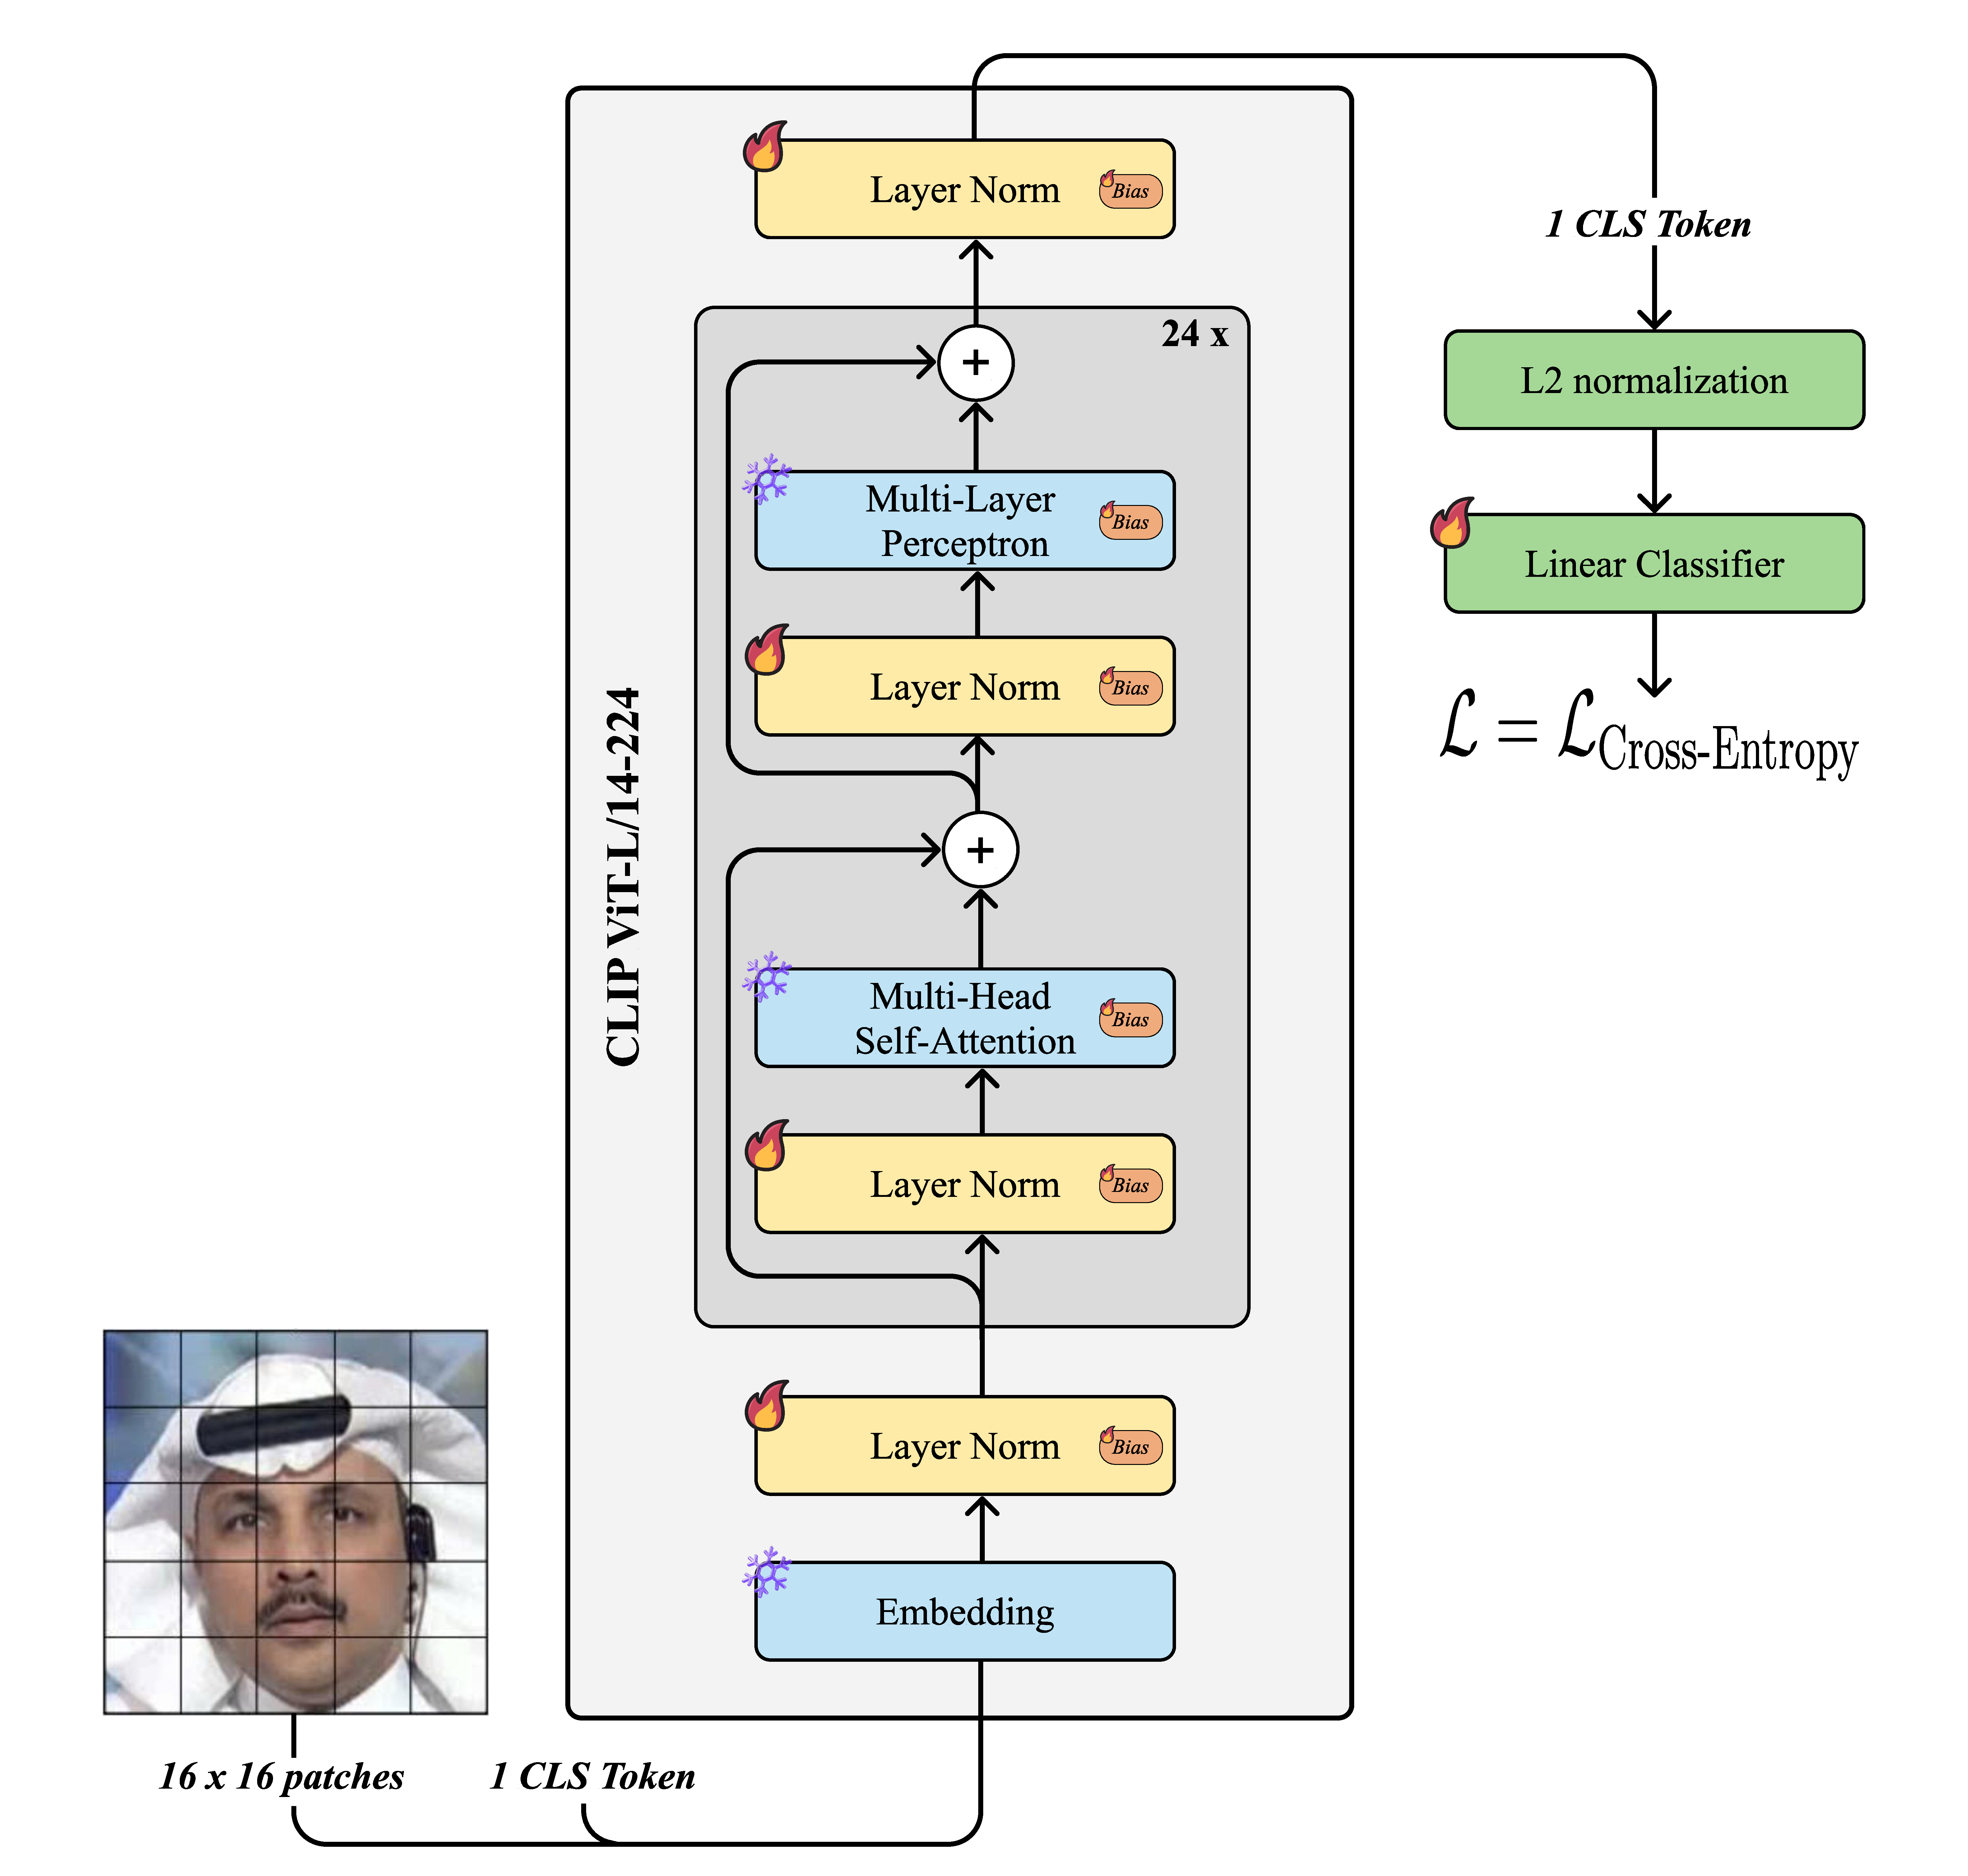
\includegraphics[width=\linewidth]{figs/biasln_overview.pdf}
    \caption{Overview of the proposed method.
The CLIP ViT-L/14 backbone is kept frozen except for its bias terms, and the extracted features are passed to a lightweight classifier for deepfake detection. During training, the features of real images are also anchored to those of the frozen encoder (Sec.~\ref{sec:ra}).}
    \label{fig:model}
\end{figure}

\subsection{Feature Extractor}

Given an input image $\mathbf{x}$, the CLIP visual encoder~\cite{radford2021clip_vitl} extracts a global feature representation
\begin{equation}
\mathbf{f} = g_{\theta}(\mathbf{x}),
\end{equation}
where $\mathbf{f} \in \mathbb{R}^{1024}$ denotes the class-token output after the final LayerNorm.
All weight matrices of $g_{\theta}$---the attention projections and the feed-forward weights---remain frozen during training, and adaptation to the deepfake detection task is delegated to the bias terms.

\subsection{Bias-only Tuning}
\label{sec:biasln}

Following BitFit~\cite{benzaken2022bitfit}, we restrict the trainable parameters of the encoder to its bias terms.
For a linear projection layer receiving an input $\mathbf{u} \in \mathbb{R}^{d}$, the output $\mathbf{h} \in \mathbb{R}^{k}$ is
\begin{equation}
    \mathbf{h} = \mathbf{W}\mathbf{u} + \mathbf{b},
\end{equation}
where $\mathbf{W} \in \mathbb{R}^{k \times d}$ is the weight matrix and $\mathbf{b} \in \mathbb{R}^{k}$ is the bias vector.
Under bias-only tuning, the weight matrix is frozen to its pre-trained state and only the bias is optimized:
\begin{equation}
    \mathbf{h} = \mathbf{W}_{\text{pt}}\mathbf{u} + \mathbf{b}_{\text{tuned}}.
\end{equation}
Each of the 24 transformer blocks has six linear layers (query, key, value and output projections of self-attention, and the two MLP layers fc1 and fc2) and two LayerNorms
\begin{equation}
    \mathrm{LN}(\mathbf{u}) = \boldsymbol{\gamma} \odot \frac{\mathbf{u} - \mu}{\sqrt{\sigma^2 + \epsilon}} + \boldsymbol{\beta},
    \label{eq:ln}
\end{equation}
where $\mu$ and $\sigma^2$ are the mean and variance of $\mathbf{u}$ across the feature dimension and $\boldsymbol{\gamma},\boldsymbol{\beta} \in \mathbb{R}^{d}$ are the affine scale and shift.
As in BitFit, we treat every additive bias vector as a bias, including the LayerNorm shifts $\boldsymbol{\beta}$, and keep the scales $\boldsymbol{\gamma}$ frozen. This gives 272{,}384 trainable encoder parameters, 0.09\% of the 303M parameters of the encoder. The BiasLN model of our first version additionally tunes $\boldsymbol{\gamma}$ (51{,}200 parameters); the following two facts explain why this brings no benefit.

\begin{proposition}[Key bias is redundant~\cite{namazifar2023bias}]
\label{prop:key}
In softmax attention with scores $s_{ij}=\mathbf{q}_i^\top(\mathbf{W}_k\mathbf{u}_j+\mathbf{b}_k)/\sqrt{d}$, the term $\mathbf{q}_i^\top\mathbf{b}_k/\sqrt{d}$ is the same for every key $j$ and cancels in the softmax. The attention output therefore does not depend on $\mathbf{b}_k$, and $\partial\mathcal{L}/\partial\mathbf{b}_k=\mathbf{0}$.
\end{proposition}

\begin{proposition}[LayerNorm shift is a tied bias update]
\label{prop:fold}
In a pre-norm block, changing the shift of the first LayerNorm by $\Delta\boldsymbol{\beta}$ changes the query, key and value outputs exactly as changing their biases by $(\mathbf{W}_q\Delta\boldsymbol{\beta},\mathbf{W}_k\Delta\boldsymbol{\beta},\mathbf{W}_v\Delta\boldsymbol{\beta})$, because $\mathbf{W}(\boldsymbol{\gamma}\odot\hat{\mathbf{u}}+\boldsymbol{\beta}+\Delta\boldsymbol{\beta})+\mathbf{b}=\mathbf{W}(\boldsymbol{\gamma}\odot\hat{\mathbf{u}}+\boldsymbol{\beta})+(\mathbf{b}+\mathbf{W}\Delta\boldsymbol{\beta})$. Likewise, the shift of the second LayerNorm acts as the bias update $\mathbf{W}_{\mathrm{fc1}}\Delta\boldsymbol{\beta}$ of fc1.
\end{proposition}
\label{sec:analysis}
We verified numerically that the key-bias gradients of our model are zero (unit test in the released code). By Proposition~\ref{prop:fold}, LayerNorm shift tuning is contained in bias tuning, and the only capability that LayerNorm tuning adds is the per-channel scale $\boldsymbol{\gamma}$. Bias tuning, LayerNorm tuning and their combination all change the network mainly through additive shifts of pre-activations, so similar behaviour is expected; Sec.~\ref{sec:roles} confirms this empirically.

\subsection{Real Anchoring}
\label{sec:ra}

Real faces from FaceForensics++, Celeb-DF, DFDC or any other source are samples of one distribution, natural face images, which the pre-trained encoder already represents consistently. Fakes are produced by many different methods and have no common distribution. Fine-tuning on one source dataset moves the features of \emph{both} classes towards source-specific statistics, such as the compression and capture pipeline of FaceForensics++. Real faces from a new dataset then no longer fall where the classifier expects real faces.

Real Anchoring prevents this drift for real images only. Let $g_{\theta_0}$ be a frozen copy of the pre-trained encoder and $\mathcal{R}$ the set of real images in a mini-batch. RA adds the loss
\begin{equation}
\mathcal{L}_{\mathrm{RA}}=\frac{1}{|\mathcal{R}|}\sum_{\mathbf{x}\in\mathcal{R}}\Big(1-\cos\big(g_\theta(\mathbf{x}),\,g_{\theta_0}(\mathbf{x})\big)\Big),
\label{eq:ra}
\end{equation}
while fake images receive no such constraint. The classifier can then separate the classes mainly by moving fake features away from the preserved real cluster.
The frozen copy $g_{\theta_0}$ runs without gradients and only on the real images of each batch (about one fifth of a FaceForensics++ batch). It is discarded after training, so the deployed model, its parameter count and its inference cost are those of the bias-tuned encoder.

\subsection{Classification Head and Training Objective}

The $L_2$-normalized feature is used as the input to a linear binary classifier:
\begin{equation}
\tilde{\mathbf{f}} = \frac{\mathbf{f}}{\lVert \mathbf{f} \rVert_2}, \qquad
\mathbf{z} = h_{\phi}(\tilde{\mathbf{f}}) = \mathbf{W}_h\tilde{\mathbf{f}}+\mathbf{b}_h,
\end{equation}
where $\mathbf{z} \in \mathbb{R}^2$ are the logits for the real ($y=0$) and fake ($y=1$) classes and $p_{i,c}=\mathrm{softmax}(\mathbf{z}_i)_c$. The fake probability $p_{i,1}$ is the detection score.
The classification loss is the class-weighted cross-entropy with label smoothing:
\begin{equation}
\begin{aligned}
\mathcal{L}_{\mathrm{ce}}&=\frac{\sum_{i=1}^{N}\sum_{c\in\{0,1\}}-\,w_c\,\tilde{y}_{i,c}\log p_{i,c}}{\sum_{i=1}^{N}w_{y_i}},\\
\tilde{y}_{i,c}&=(1-\alpha)\,\mathbb{1}[c=y_i]+\tfrac{\alpha}{2},
\end{aligned}
\label{eq:ce}
\end{equation}
with class weights $w_0=1$ (real) and $w_1=2$ (fake) to compensate for the class imbalance of FF++, and smoothing $\alpha=0.1$. The normalization by $\sum_i w_{y_i}$ is the convention of PyTorch's \texttt{CrossEntropyLoss}.
The full training objective is
\begin{equation}
\mathcal{L}=\mathcal{L}_{\mathrm{ce}}+\lambda\,\mathcal{L}_{\mathrm{RA}},
\label{eq:total}
\end{equation}
with $\lambda=1$; $\lambda=0$ recovers plain bias tuning.

\subsection{Training and Data Setup}
\label{sec:impl}

Our model is trained on the FaceForensics++ (FF++) dataset under the c23 compression setting and evaluated under cross-dataset and cross-method protocols.

\noindent\textbf{Data Preprocessing.}\par
We follow the standard dataset preprocessing protocol proposed in DeepfakeBench~\cite{yan2023deepfakebench}, which consists of the following steps:
\begin{itemize}[leftmargin=*, topsep=2pt, itemsep=2pt, label=--]
    \item Sample 32 frames evenly from each video.
    \item Extract the largest face in each frame using RetinaFace~\cite{deng2020retinaface}.
    \item Align the detected face using the predicted facial landmarks.
    \item Enlarge the bounding box of the aligned face by a factor of $1.3\times$.
    \item Crop the face region, resize it to $224 \times 224$ and save it in lossless format.
\end{itemize}
For training, 8 evenly spaced frames of every video are used; at test time all 32 frames are scored.

\noindent\textbf{Data Augmentation.}\par
We follow the DeepfakeBench~\cite{yan2023deepfakebench} augmentation pipeline implemented with the \texttt{Albumentations} library. Each of the following is applied with probability 0.5:
\begin{itemize}[leftmargin=*, topsep=2pt, itemsep=2pt, label=--]
    \item Horizontal flipping,
    \item Random rotation (range $[-10, 10]$ degrees),
    \item Gaussian blur (kernel range $[3, 7]$),
    \item One of brightness/contrast adjustment (range $[-0.1, 0.1]$), FancyPCA, or hue/saturation jitter,
    \item JPEG compression (quality range $[40, 100]$),
\end{itemize}
followed by isotropic resizing to $224\times224$.

\noindent\textbf{Training Configuration and Optimization.}\par
All variants are trained for 10 epochs with a batch size of 32 on one NVIDIA A100-40GB GPU with bfloat16 autocast.
We use the Adam optimizer with $\beta_1 = 0.9$, $\beta_2 = 0.999$, an initial learning rate of $3 \times 10^{-4}$, and zero weight decay.
The learning rate follows a cosine annealing schedule with $T_{\max}=10$ epochs and a minimum learning rate of $1 \times 10^{-5}$.
Full fine-tuning uses a learning rate of $10^{-5}$ for the encoder and $3\times10^{-4}$ for the head; GenD and Effort use the hyper-parameters of their authors (Sec.~\ref{sec:protocol}). The checkpoint with the highest frame-level AUC on the FF++ validation split is kept.


\section{Experiments}
\subsection{Datasets}
\label{sec:datasets}
\label{sec:protocol}

Our model is evaluated in three protocols: \textit{in-domain}, \textit{cross-dataset}, and \textit{cross-method}.
Table~\ref{tab:datasets} summarizes the datasets, their roles, and the number of forgery methods.
Here, \textbf{NoGenMethod} denotes the number of forgery generation methods in each dataset.

\begin{table}[h]
  \centering
  \caption{Datasets used for training and evaluation.
NoGenMethod denotes the number of forgery methods in each dataset.}
  \label{tab:datasets}
  \small
  \setlength{\tabcolsep}{2pt}
  \renewcommand{\arraystretch}{1.1}
  \resizebox{\columnwidth}{!}{
  \begin{tabular}{@{} l c c c >{\raggedright\arraybackslash} m{0.45\columnwidth} @{}}
    \toprule
    \raisebox{0.6\normalbaselineskip}{\textbf{Dataset}} &
    \raisebox{0.6\normalbaselineskip}{\textbf{Year}} &
    \raisebox{0.6\normalbaselineskip}{\textbf{Role}} &
    \multicolumn{1}{c}{\textbf{\shortstack[c]{NoGen-\\Method}}} &
    \multicolumn{1}{c@{}}{\raisebox{0.6\normalbaselineskip}{\textbf{Description}}} \\
    \midrule
    \textbf{FF++}~\cite{rossler2019ff} & 2019 & In-domain & 4 & Main training set with four classical forgery types. \\
    \midrule
    \textbf{CDF-v2}~\cite{li2020celeb} & 2020 & Cross-dataset & 1 & High-quality forgeries with subtle real--fake differences.\\
    \textbf{DFD}~\cite{dufour2019dfd} & 2019 & Cross-dataset & 5 & Diverse capture conditions and environments.\\
    \textbf{DFDCP}~\cite{dolhansky2019dfdcp} & 2019 & Cross-dataset & 8 & Preview set with quality variation and extra noise.\\
    \textbf{DFDC}~\cite{dolhansky2020dfdc} & 2019 & Cross-dataset & 8 & Large-scale benchmark with compression and real-world variability.\\
    \midrule
    \textbf{DF40}~\cite{yan2024df40} & 2024 & Cross-method & 40 & Broad benchmark for cross-method evaluation.\\
    \bottomrule
  \end{tabular}
  }
\end{table}

\textbf{1. In-domain evaluation:}
All models are trained exclusively on the four classical manipulations of FaceForensics++ (FF++) under the HQ compression setting (c23), using the official 720/140/140 video split, and tested on the FF++ test split.

\textbf{2. Cross-dataset evaluation:}
Following the protocol of Effort~\cite{yan2025effort}, the trained model is evaluated on four unseen datasets: CDF-v2, DFD, DFDCP, and DFDC.
These benchmarks differ substantially in scale, visual quality, acquisition conditions, and forgery diversity, thereby producing different levels of distribution shift with respect to the training data.

\textbf{3. Cross-method evaluation:}
We further evaluate generalization to unseen forgery methods on DF40~\cite{yan2024df40}, a recent benchmark covering 40 manipulation methods.
We use seven advanced face-swapping methods of DF40, namely UniFace, BlendFace, E4S, FaceDancer, FSGAN, InSwap, and SimSwap, each applied to FF++ identities and paired with the FF++ real test videos.

\noindent\textbf{Checkpoint selection.}\label{sec:selection}
When generalization is the goal, the chosen checkpoint has a large effect on the reported numbers, and prior work handles this step differently. Effort~\cite{yan2025effort} does not state a selection rule; it builds on the DeepfakeBench code~\cite{yan2023deepfakebench}, whose trainer evaluates every test dataset after each epoch and keeps a best checkpoint for each of them. GenD~\cite{yermakov2025gend} selects on a custom validation set drawn from the training or validation splits of other datasets, several of which are also among its test benchmarks (with disjoint samples). The first version of this manuscript selected on a subset of CDF-v2, which is also a test dataset. Selection that uses data from the target domains makes cross-dataset results optimistic. In this revision, every method, including all baselines, therefore selects its checkpoint on the FF++ \emph{validation} split only; an automated audit (released with the code) confirms that this split shares no frame and no video with any test set.

\noindent\textbf{Baselines.}
We re-implemented GenD (LayerNorm tuning, $L_2$ normalization, cross-entropy plus $0.1\times$ alignment and $0.5\times$ uniformity loss, learning rate $2\times10^{-4}$, batch size 16) and Effort (rank-1 SVD residual on all attention projections, learning rate $2\times10^{-4}$, weight decay $5\times10^{-4}$, batch size 16) following their released code, and trained them with our data, augmentation and selection rule. Methods that we could not re-train are reported with the numbers published by their authors.

\subsection{Evaluation Benchmark}

To ensure fair comparison with prior state-of-the-art methods, we adopt the Area Under the ROC Curve (AUC) as the primary evaluation metric.
Following recent deepfake detection benchmarks, we report \textit{video-level AUC}, where the prediction score of a video is the average of the fake probabilities of its 32 sampled frames.
Avg(D) and Avg(M) denote the means over the four cross-dataset and the seven cross-method test sets.
Each re-trained configuration is run with several random seeds ($n$ in the tables); we report the mean and the sample standard deviation over seeds, and test differences with a paired $t$-test across seeds and the DeLong test~\cite{delong1988} on the seed-averaged scores.

\subsection{Results}
\label{sec:main}

Tables~\ref{tab:in_domain_val}, \ref{tab:comparison} and~\ref{tab:main} report the in-domain, published and re-trained results.

\begin{table}[H]
\centering
\caption{In-domain video AUC (\%) on the four manipulation subsets of the FF++ c23 test set (seed means, all models re-trained under our protocol).}
\label{tab:in_domain_val}
\label{tab:indomain}
\resizebox{\columnwidth}{!}{% generated by tools/paper_assets.py -- do not edit
\begin{tabular}{l cccc c}
\toprule
\textbf{Method} & \textbf{DF} & \textbf{F2F} & \textbf{FS} & \textbf{NT} & \textbf{Mean} \\
\midrule
Effort~\cite{yan2025effort} & \textbf{100.0} & 99.1 & 99.3 & 97.8 & \cellcolor{gray!15}99.1 \\
GenD~\cite{yermakov2025gend} & \textbf{100.0} & 98.9 & 99.2 & 96.3 & 98.6 \\
BiasLN (bias + LN) & \textbf{100.0} & \textbf{99.6} & \cellcolor{gray!15}99.6 & \textbf{98.8} & \textbf{99.5} \\
Bias only (BitFit) & \textbf{100.0} & \textbf{99.6} & \textbf{99.8} & \cellcolor{gray!15}98.7 & \textbf{99.5} \\
\midrule
RA (Ours) & \cellcolor{gray!15}99.9 & \cellcolor{gray!15}99.5 & 99.1 & 97.9 & \cellcolor{gray!15}99.1 \\
\bottomrule
\end{tabular}
}
\end{table}

\begin{table*}[t]
\centering
\captionsetup{labelsep=period, labelfont=bf, hypcap=false}
\caption{Benchmarking results of cross-dataset evaluations (Protocol-2) and cross-method evaluations (Protocol-3).
All detectors are trained on FF++ c23~\cite{rossler2019ff} and evaluated on other fake data.
The results of other methods are taken from Table~1 of Effort~\cite{yan2025effort}, and the Forensics Adapter and GenD rows from their papers; $\dagger$ marks the authors' released checkpoints.
These numbers come from different training recipes and checkpoint-selection rules (Sec.~\ref{sec:selection}), whereas our row is selected on FF++ validation only and averaged over $n$ seeds. Bold: best; shaded: second best.}
\label{tab:comparison}
\label{tab:literature}
\vspace{2mm}
\resizebox{\textwidth}{!}{% generated by tools/paper_assets.py -- do not edit
\begin{tabular}{l r ccccc cccccccc}
\toprule
\multirow{2}{*}{\textbf{Method}} & \multirow{2}{*}{\textbf{Trainable Params}} & \multicolumn{5}{c}{\textbf{Cross-dataset}} & \multicolumn{8}{c}{\textbf{Cross-method}} \\
\cmidrule(lr){3-7} \cmidrule(lr){8-15}
& & \textbf{CDF-v2} & \textbf{DFD} & \textbf{DFDC} & \textbf{DFDCP} & \textbf{Avg(D)} & \textbf{UniFace} & \textbf{BlendFace} & \textbf{E4S} & \textbf{FaceDan.} & \textbf{FSGAN} & \textbf{InSwap} & \textbf{SimSwap} & \textbf{Avg(M)} \\
\midrule
F3Net~\cite{qian2020frequency} & 22M & 0.789 & 0.844 & 0.718 & 0.749 & 0.775 & 0.809 & 0.808 & 0.494 & 0.717 & 0.845 & 0.757 & 0.674 & 0.729 \\
SPSL~\cite{liu2021spsl} & 21M & 0.799 & 0.871 & 0.724 & 0.770 & 0.791 & 0.747 & 0.748 & 0.514 & 0.666 & 0.812 & 0.643 & 0.665 & 0.685 \\
SRM~\cite{luo2021srm} & 55M & 0.840 & 0.885 & 0.695 & 0.728 & 0.787 & 0.749 & 0.704 & 0.704 & 0.659 & 0.772 & 0.793 & 0.694 & 0.725 \\
CORE~\cite{ni2022core} & 22M & 0.809 & 0.882 & 0.721 & 0.720 & 0.783 & 0.871 & 0.843 & 0.679 & 0.774 & 0.958 & 0.855 & 0.724 & 0.815 \\
RECCE~\cite{cao2022recce} & 48M & 0.823 & 0.891 & 0.696 & 0.734 & 0.786 & 0.898 & 0.832 & 0.683 & 0.848 & 0.949 & 0.848 & 0.768 & 0.832 \\
SLADD~\cite{chen2022sladd} & 21M & 0.837 & 0.904 & 0.772 & 0.756 & 0.817 & 0.878 & 0.882 & 0.765 & 0.825 & 0.943 & 0.879 & 0.794 & 0.852 \\
SBI~\cite{shiohara2022sbi} & 18M & 0.886 & 0.827 & 0.717 & 0.848 & 0.820 & 0.724 & 0.891 & 0.750 & 0.594 & 0.803 & 0.712 & 0.701 & 0.739 \\
UCF~\cite{yan2023ucf} & 47M & 0.837 & 0.867 & 0.742 & 0.770 & 0.804 & 0.831 & 0.827 & 0.731 & 0.862 & 0.937 & 0.809 & 0.647 & 0.806 \\
IID~\cite{huang2023iid} & 66M & 0.838 & 0.939 & 0.700 & 0.689 & 0.791 & 0.839 & 0.789 & 0.766 & 0.844 & 0.927 & 0.789 & 0.644 & 0.800 \\
LSDA$^\dagger$~\cite{yan2024latent} & 133M & 0.875 & 0.881 & 0.701 & 0.812 & 0.817 & 0.872 & 0.875 & 0.694 & 0.721 & 0.939 & 0.855 & 0.793 & 0.821 \\
ProDet$^\dagger$~\cite{cheng2024prodet} & 96M & 0.926 & 0.901 & 0.707 & 0.828 & 0.840 & 0.908 & \cellcolor{gray!15}0.929 & 0.771 & 0.747 & 0.928 & 0.837 & 0.844 & 0.852 \\
CDFA$^\dagger$~\cite{lin2024cdfa} & 87M & 0.938 & 0.954 & 0.830 & 0.881 & 0.901 & 0.762 & 0.756 & 0.631 & 0.803 & 0.942 & 0.772 & 0.757 & 0.775 \\
Effort~\cite{yan2025effort} & 0.19M & 0.956 & 0.965 & 0.843 & 0.909 & 0.918 & 0.962 & 0.873 & 0.983 & 0.926 & 0.957 & 0.936 & 0.926 & 0.938 \\
Forensics Adapter~\cite{cui2025forada} & 5.7M & \cellcolor{gray!15}0.957 & \cellcolor{gray!15}0.972 & \cellcolor{gray!15}0.872 & \textbf{0.928} & \textbf{0.932} & 0.950 & 0.880 & 0.968 & 0.945 & 0.975 & 0.948 & 0.912 & 0.940 \\
GenD~\cite{yermakov2025gend} & 0.1M & \textbf{0.960} & 0.970 & 0.870 & \cellcolor{gray!15}0.917 & \cellcolor{gray!15}0.929 & \textbf{0.983} & \textbf{0.933} & \cellcolor{gray!15}0.988 & \cellcolor{gray!15}0.954 & \cellcolor{gray!15}0.982 & \textbf{0.965} & \textbf{0.958} & \textbf{0.966} \\
\midrule
RA (Ours) ($n{=}1$) & 0.27M & 0.954 & \textbf{0.984} & \textbf{0.883} & 0.896 & \cellcolor{gray!15}0.929 & \cellcolor{gray!15}0.973 & 0.897 & \textbf{0.991} & \textbf{0.972} & \textbf{0.983} & \cellcolor{gray!15}0.963 & \cellcolor{gray!15}0.953 & \cellcolor{gray!15}0.962 \\
\bottomrule
\end{tabular}
}
\end{table*}

\begin{table*}[t]
\centering
\captionsetup{labelsep=period, labelfont=bf, hypcap=false}
\caption{Video AUC of re-trained methods under the same protocol (FF++ c23 training, checkpoint selected on the FF++ validation split). Avg(D) and Avg(M) are mean $\pm$ standard deviation over $n$ seeds; per-dataset values are seed means. Params: trainable parameters of the deployed model. Bold: best; shaded: second best.}
\label{tab:main}
\vspace{2mm}
\resizebox{\textwidth}{!}{% generated by tools/paper_assets.py -- do not edit
\begin{tabular}{l r c ccccc cccccccc}
\toprule
\multirow{2}{*}{\textbf{Method}} & \multirow{2}{*}{\textbf{Params}} & \multirow{2}{*}{$n$} & \multicolumn{5}{c}{\textbf{Cross-dataset}} & \multicolumn{8}{c}{\textbf{Cross-method}} \\
\cmidrule(lr){4-8} \cmidrule(lr){9-16}
& & & \textbf{CDF-v2} & \textbf{DFD} & \textbf{DFDC} & \textbf{DFDCP} & \textbf{Avg(D)} & \textbf{UniFace} & \textbf{BlendFace} & \textbf{E4S} & \textbf{FaceDan.} & \textbf{FSGAN} & \textbf{InSwap} & \textbf{SimSwap} & \textbf{Avg(M)} \\
\midrule
Effort~\cite{yan2025effort} & 0.199M & 2 & 0.946 & 0.979 & 0.844 & 0.880 & 0.912\,{\scriptsize$\pm$0.001} & 0.971 & \cellcolor{gray!15}0.916 & 0.988 & \textbf{0.976} & 0.979 & 0.953 & 0.938 & 0.960\,{\scriptsize$\pm$0.008} \\
GenD~\cite{yermakov2025gend} & 0.104M & 2 & \cellcolor{gray!15}0.951 & \cellcolor{gray!15}0.980 & \cellcolor{gray!15}0.862 & 0.900 & \cellcolor{gray!15}0.923\,{\scriptsize$\pm$0.003} & \textbf{0.980} & 0.913 & \cellcolor{gray!15}0.990 & 0.959 & 0.980 & \textbf{0.966} & \textbf{0.962} & \textbf{0.964\,{\scriptsize$\pm$0.003}} \\
BiasLN (bias + LN) & 0.326M & 2 & \cellcolor{gray!15}0.951 & 0.974 & 0.853 & \textbf{0.916} & \cellcolor{gray!15}0.923\,{\scriptsize$\pm$0.009} & 0.960 & \textbf{0.924} & 0.984 & \cellcolor{gray!15}0.974 & \cellcolor{gray!15}0.982 & 0.951 & 0.932 & 0.958\,{\scriptsize$\pm$0.007} \\
Bias only (BitFit) & 0.274M & 1 & 0.949 & 0.973 & 0.834 & \cellcolor{gray!15}0.903 & 0.915 & 0.967 & \textbf{0.924} & 0.978 & 0.968 & 0.977 & 0.958 & 0.940 & 0.959 \\
\midrule
RA (Ours) & 0.274M & 1 & \textbf{0.954} & \textbf{0.984} & \textbf{0.883} & 0.896 & \textbf{0.929} & \cellcolor{gray!15}0.973 & 0.897 & \textbf{0.991} & 0.972 & \textbf{0.983} & \cellcolor{gray!15}0.963 & \cellcolor{gray!15}0.953 & \cellcolor{gray!15}0.962 \\
\bottomrule
\end{tabular}
}
\end{table*}

On the \textbf{in-domain} FF++ evaluation in Table~\ref{tab:in_domain_val}, all parameter-efficient variants are close to saturation, so in-domain accuracy does not discriminate between them; RA trades a small in-domain decrease for its cross-domain gain.

In the \textbf{cross-dataset} and \textbf{cross-method} evaluations against published results (Table~\ref{tab:comparison}), RA reaches an Avg(D) of \num{AvgDRaReal} and an Avg(M) of \num{AvgMRaReal}, in the range of the strongest CLIP-based detectors, even though its checkpoint is never selected on target-domain data.

Under the common protocol (Table~\ref{tab:main}), bias tuning, LayerNorm tuning and BiasLN reach similar averages. Real Anchoring raises the cross-dataset average of bias tuning from \num{AvgDBitfit} to \num{AvgDRaReal}, with the largest gains on DFDC and DFD, while it is slightly below plain bias tuning on DFDCP. \pending{Final wording after seeds 1 and 2: state which differences are significant (paired t-test, DeLong) and avoid ``outperforms'' where they are not; describe full FT and linear probe once their runs finish.}


\subsection{Feature-Space Comparison on Celeb-DF-v2}
\label{sec:drift}

\begin{figure*}[t]
    \centering
    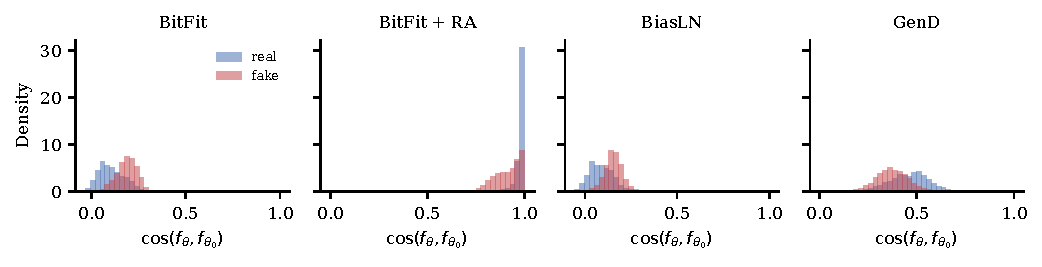
\includegraphics[width=0.72\textwidth]{generated/fig_drift.pdf}
    \caption{Distribution of the cosine similarity between tuned and frozen-encoder features for real and fake frames of the unseen CDF-v2 test set (seed 1024). Values near 1 mean that the pre-trained representation is preserved.}
    \label{fig:drift}
\end{figure*}

\begin{figure*}[t]
    \centering
    \captionsetup{justification=centering}
    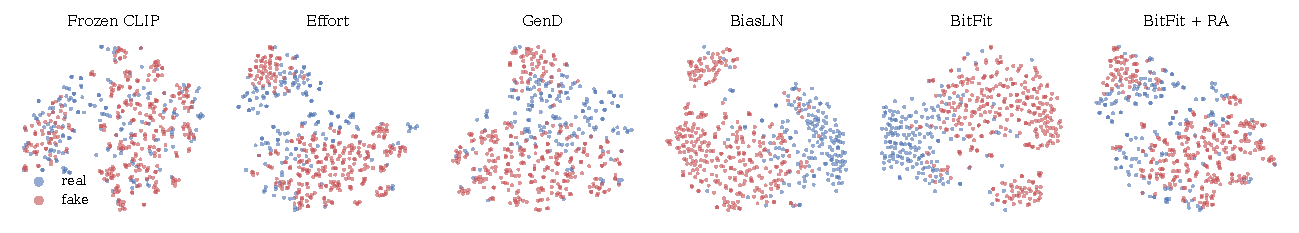
\includegraphics[width=0.9\textwidth]{generated/fig_tsne.pdf}
    \caption{T-SNE visualization of video-level real and fake feature embeddings from the Celeb-DF-v2 test set for the frozen encoder and the tuned models (mean over 8 frames, seed 1024).}
    \label{fig:tsne}
    \label{fig:celebdf-feature-comparison}
\end{figure*}

To see what RA changes, we compare the features of the tuned encoders with those of the frozen encoder on the unseen CDF-v2 test set (8 frames per video). Figure~\ref{fig:drift} shows the cosine similarity $\cos(g_\theta(\mathbf{x}),g_{\theta_0}(\mathbf{x}))$ per frame. Bias tuning and BiasLN move the features of \emph{both} classes almost orthogonal to the pre-trained ones (median \num{DriftRealBitfit} for real and \num{DriftFakeBitfit} for fake frames under bias tuning). The result is nearly unchanged after removing the mean feature of each model, so this is a change of structure rather than a common offset. With RA, real CDF-v2 frames, which were never seen during training, stay close to their pre-trained features (median \num{DriftRealRaReal}), while fake frames move further (median \num{DriftFakeRaReal}). The anchoring learned on FF++ real faces thus transfers to real faces of another dataset, which is the behaviour RA was designed for; GenD lies in between. Figure~\ref{fig:tsne} shows t-SNE embeddings of the video-level features.


\subsection{Ablation Study}
\label{sec:ra-results}

We conduct an ablation study to isolate the effect of Real Anchoring, as summarized in Table~\ref{tab:ablation}.
All rows share the data, classifier, schedule and selection rule, and differ in one factor at a time: whether $\mathcal{L}_{\mathrm{RA}}$ is used, which images are anchored, the weight $\lambda$, and whether LayerNorm scales are tuned in addition to the biases.

\begin{table*}[t]
  \centering
  \captionsetup{labelsep=period, labelfont=bf, hypcap=false}
  \caption{Ablation of Real Anchoring. $\mathcal{L}_{\mathrm{RA}}$: with (\ding{51}) or without (\ding{55}) the anchoring loss; Anchored: images whose features are anchored to the frozen encoder; $\lambda$: weight of the anchoring loss in Eq.~\eqref{eq:total}. Video AUC; Avg(D) and Avg(M) are mean $\pm$ standard deviation over $n$ seeds. Bold: best; shaded: second best.}
  \label{tab:ablation}
  \label{tab:anchor}
  \small
  \resizebox{0.85\textwidth}{!}{% generated by tools/paper_assets.py -- do not edit
\begin{tabular}{l c c c c cccc c c}
\toprule
\multirow{2}{*}{\textbf{Tuned params}} & \multirow{2}{*}{$\mathcal{L}_{\mathrm{RA}}$} & \multirow{2}{*}{\textbf{Anchored}} & \multirow{2}{*}{$\lambda$} & \multirow{2}{*}{$n$} & \multicolumn{4}{c}{\textbf{Cross-dataset}} & \multirow{2}{*}{\textbf{Avg(D)}} & \multirow{2}{*}{\textbf{Avg(M)}} \\
\cmidrule(lr){6-9}
& & & & & \textbf{CDF-v2} & \textbf{DFD} & \textbf{DFDC} & \textbf{DFDCP} & & \\
\midrule
BiasLN (bias + LN) & \ding{55} & -- & -- & 2 & 0.951 & 0.974 & 0.853 & \textbf{0.916} & \cellcolor{gray!15}0.923\,{\scriptsize$\pm$0.009} & 0.958\,{\scriptsize$\pm$0.007} \\
\midrule
Bias only & \ding{55} & -- & -- & 1 & 0.949 & 0.973 & 0.834 & \cellcolor{gray!15}0.903 & 0.915 & 0.959 \\
Bias only & \ding{51} & fake & 1 & 1 & 0.949 & 0.977 & 0.877 & 0.888 & \cellcolor{gray!15}0.923 & \cellcolor{gray!15}0.962 \\
Bias only & \ding{51} & all & 1 & 1 & 0.943 & 0.977 & 0.871 & 0.893 & 0.921 & 0.961 \\
Bias only & \ding{51} & real & 0.3 & 1 & \cellcolor{gray!15}0.953 & \cellcolor{gray!15}0.982 & 0.864 & 0.890 & 0.922 & \textbf{0.968} \\
Bias only & \ding{51} & real & 3 & 1 & 0.924 & 0.978 & \cellcolor{gray!15}0.879 & 0.871 & 0.913 & 0.936 \\
\midrule
\textbf{Bias only (Ours)} & \ding{51} & real & 1 & 1 & \textbf{0.954} & \textbf{0.984} & \textbf{0.883} & 0.896 & \textbf{0.929} & \cellcolor{gray!15}0.962 \\
\bottomrule
\end{tabular}
}
\end{table*}

\noindent\textbf{With and without $\mathcal{L}_{\mathrm{RA}}$.}
Adding the anchoring loss to bias tuning raises Avg(D) from \num{AvgDBitfit} to \num{AvgDRaReal} and Avg(M) from \num{AvgMBitfit} to \num{AvgMRaReal}. \pending{BiasLN with and without RA (run in progress).}

\noindent\textbf{Which images to anchor.}
Anchoring helps whichever images are anchored, because keeping features close to the encoder limits overfitting to FF++. Anchoring \emph{only real} images gives the largest cross-dataset gain, while anchoring all images (\num{AvgDRaAll}) or only fake images (\num{AvgDRaFake}) gives smaller gains, which supports the asymmetric view of Sec.~\ref{sec:ra}.

\noindent\textbf{Anchoring strength.}
A weaker anchor ($\lambda=0.3$, Avg(D) \num{AvgDRaRealLAD}) keeps part of the cross-dataset gain and gives the highest cross-method average (\num{AvgMRaRealLAD}), and a stronger one ($\lambda=3$, \num{AvgDRaRealLD}) constrains the features too much and lowers both the cross-dataset and the cross-method averages; we use $\lambda=1$ throughout.

\noindent\textbf{Which parameters to tune.}
\label{sec:roles}
Table~\ref{tab:roles} compares tuning schemes that differ only in the set of tuned parameters, without anchoring. Bias-only tuning matches BiasLN on unseen data, and LayerNorm-only tuning is comparable with both. Splitting the biases by role, into the content-dependent query and fc1 biases or the residual-stream translations (value, output and fc2 biases), changes the averages by less than the seed-to-seed variation. Together with Proposition~\ref{prop:fold}, these results indicate that the choice among these small additive-shift subspaces matters little, and that how the adaptation is regularized matters more.

\begin{table}[t]
\centering
\captionsetup{labelsep=period, labelfont=bf, hypcap=false}
\caption{Which parameters to tune (no anchoring). Only the tuned subset of the encoder differs. Video AUC, mean $\pm$ std over $n$ seeds.}
\label{tab:roles}
\resizebox{\columnwidth}{!}{% generated by tools/paper_assets.py -- do not edit
\begin{tabular}{l r c ccc}
\toprule
\textbf{Tuned parameters} & \textbf{\#} & $n$ & \textbf{Avg(D)} & \textbf{Avg(M)} & \textbf{FF++} \\
\midrule
All biases incl.\ LN $\beta$ (BitFit) & 272{,}384 & 1 & 0.915 & 0.959 & \textbf{0.995} \\
$\mathbf{b}_q,\mathbf{b}_{\mathrm{fc1}}$ (content-dependent) & 122{,}880 & 1 & 0.920 & 0.958 & 0.988 \\
$\mathbf{b}_v,\mathbf{b}_o,\mathbf{b}_{\mathrm{fc2}}$ (translations) & 73{,}728 & 1 & 0.915 & 0.960 & 0.993 \\
LN $\gamma,\beta$ & 51{,}200 & 1 & 0.921 & 0.959 & 0.987 \\
LN $\beta$ only & 25{,}600 & 1 & 0.914 & 0.958 & 0.985 \\
LN $\gamma$ only & 25{,}600 & 1 & 0.914 & \textbf{0.961} & 0.984 \\
BitFit + LN $\gamma$ (BiasLN) & 323{,}584 & 2 & \textbf{0.923}\,{\scriptsize$\pm$0.009} & 0.958\,{\scriptsize$\pm$0.007} & \textbf{0.995}\,{\scriptsize$\pm$0.001} \\
\bottomrule
\end{tabular}
}
\end{table}


\subsection{Computational Cost}
\label{sec:cost}
Table~\ref{tab:cost} reports measured costs on one A100-40GB with $224\times224$ inputs. Training is forward, backward and an Adam step at batch size 32; inference latency is at batch size 1. Because bias tuning changes values but not the architecture, the deployed model has exactly the cost of the frozen CLIP encoder (162 GFLOPs per image), whereas Effort and unmerged LoRA add work at every forward pass. Compared with full fine-tuning, bias tuning trains $1.42\times$ faster per step, needs 38\% less peak memory and stores an $890\times$ smaller checkpoint. Among parameter-efficient methods the training costs are similar, because back-propagation through the 24 frozen blocks dominates. RA adds one gradient-free forward pass on the real images of each batch and a frozen copy of the encoder in memory during training only.

\begin{table}[t]
\centering
\captionsetup{labelsep=period, labelfont=bf, hypcap=false}
\caption{Measured cost on an NVIDIA A100-40GB (fp32, $224\times224$). Train: batch 32, forward + backward + Adam step. Infer: batch 1. Ckpt: size of the stored trainable tensors.}
\label{tab:cost}
\resizebox{\columnwidth}{!}{%
\begin{tabular}{l r r r r r r}
\toprule
\textbf{Method} & \textbf{Trainable} & \textbf{Ckpt} & \textbf{Train} & \textbf{Train} & \textbf{Infer} & \textbf{GFLOPs} \\
 & & \textbf{(MB)} & \textbf{img/s} & \textbf{mem (GB)} & \textbf{ms} & \\
\midrule
Linear probe & 0.002M & 0.0 & 100.6 & 1.67 & 17.0 & 162.0 \\
LayerNorm (GenD) & 0.104M & 0.4 & 47.1 & 12.16 & 17.1 & 162.0 \\
Effort & 0.199M & 0.8 & 41.7 & 13.22 & 23.8 & 162.2 \\
Bias only & 0.274M & 1.1 & 46.6 & 12.16 & 17.1 & 162.0 \\
BiasLN & 0.326M & 1.3 & 46.5 & 12.16 & 17.2 & 162.0 \\
LoRA $r{=}8$ & 0.788M & 3.0 & 45.9 & 12.87 & 18.6 & 162.4 \\
Full FT & 303.2M & 1156.7 & 32.8 & 19.72 & 17.2 & 162.0 \\
\bottomrule
\end{tabular}}
\end{table}


\section{Conclusion}

In this paper, we presented Real Anchoring, an asymmetric objective that preserves the pre-trained features of real faces while a frozen CLIP encoder is adapted by tuning only its biases.
Bias tuning alone moves the features of real faces from unseen datasets almost orthogonal to their pre-trained representation. RA keeps them in place and lets the detector learn how fakes deviate from them, which improves cross-dataset generalization without adding parameters or inference cost. Anchoring all images or only fakes helps less, so the asymmetry is essential.
Under a protocol that never selects checkpoints on target-domain data, adding LayerNorm parameters to bias tuning brings no benefit, consistent with our analysis that LayerNorm shifts are tied bias updates and the key bias is redundant. \pending{final wording after significance tests over all seeds.}


\section{Limitations and Future Work}
\label{sec:limits}
Although our method is competitive with current state-of-the-art methods, it still has several limitations that should be addressed in future work.

First, all models are trained on FF++ only, and the validation split is in-domain. A validation mixture built from datasets that are not used for testing could select better checkpoints without leaking test information.

Second, our model works on cropped video frames instead of full video sequences.
Because of this, the model may miss temporal inconsistencies and motion artifacts that only appear across consecutive frames.

Third, the cross-method evaluation covers seven face-swapping methods of DF40; entire-face synthesis and diffusion-based editing are not evaluated. RA also assumes that real test faces resemble natural pre-training images; heavily processed real videos may violate this assumption, which could explain the small decrease on DFDCP.

Fourth, the CLIP ViT-L/14 backbone requires 162 GFLOPs per image, so deployment on edge devices would require distilling the detector into a smaller encoder. Strong results on public benchmarks also do not eliminate the risk of misuse: as detectors become more effective, malicious users may use their feedback to create more realistic fake content.

In future work, we will study multi-source validation strategies, incorporate temporal modeling, evaluate the method on newer manipulation techniques, and examine how it can be deployed more safely in practice.


\begin{thebibliography}{99}
\balance

\bibitem{goodfellow2020gan}
Goodfellow I, Pouget-Abadie J, Mirza M, Xu B, Warde-Farley D, Ozair S, Courville A, Bengio Y.
Generative adversarial networks.
Commun ACM. 2020;63(11):139--44.

\bibitem{yang2022diffusion}
Yang L, Zhang Z, Song Y, Hong S, Xu R, Zhao Y, Zhang W, Cui B, Yang MH.
Diffusion models: A comprehensive survey of methods and applications.
ACM Comput Surv. 2023;56(4):1--39. doi:10.1145/3626235.

\bibitem{yan2023deepfakebench}
Yan Z, Zhang Y, Yuan X, Lyu S, Wu B.
DeepfakeBench: A comprehensive benchmark of deepfake detection.
Adv Neural Inf Process Syst (NeurIPS), Datasets and Benchmarks Track. 2023;36:4534--65.

\bibitem{radford2021clip_vitl}
Radford A, Kim JW, Hallacy C, Ramesh A, Goh G, Agarwal S, et al.
Learning transferable visual models from natural language supervision.
In: Proc Int Conf Mach Learn (ICML). 2021;8748--63.

\bibitem{ojha2023universal}
Ojha U, Li Y, Lee YJ.
Towards universal fake image detectors that generalize across generative models.
In: Proc IEEE/CVF Conf Comput Vis Pattern Recognit (CVPR). 2023;24480--9.

\bibitem{kumar2022finetuning}
Kumar A, Raghunathan A, Jones R, Ma T, Liang P.
Fine-tuning can distort pretrained features and underperform out-of-distribution.
In: Int Conf Learn Represent (ICLR). 2022.

\bibitem{yan2025effort}
Yan Z, Wang J, Jin P, Zhang KY, Liu C, Chen S, et al.
Orthogonal subspace decomposition for generalizable AI-generated image detection.
In: Proc Int Conf Mach Learn (ICML). 2025.

\bibitem{yermakov2025gend}
Yermakov A, Cech J, Matas J, Fritz M.
Deepfake detection that generalizes across benchmarks.
In: Proc IEEE/CVF Winter Conf Appl Comput Vis (WACV). 2026;773--83.

\bibitem{cui2025forada}
Cui X, Li Y, Luo A, Zhou J, Dong J.
Forensics Adapter: Adapting CLIP for generalizable face forgery detection.
In: Proc IEEE/CVF Conf Comput Vis Pattern Recognit (CVPR). 2025;19207--17.

\bibitem{xu2026bpl}
Xu Y, He R, Yan Z, Dong Y, Han Z, Wang X, Yin Y.
BPL: Generalizable deepfake detection via bias-only pair-aware learning.
In: Proc Int Conf Mach Learn (ICML). 2026.

\bibitem{rossler2019ff}
R{\"o}ssler A, Cozzolino D, Verdoliva L, Riess C, Thies J, Nie{\ss}ner M.
FaceForensics++: Learning to detect manipulated facial images.
In: Proc IEEE/CVF Int Conf Comput Vis (ICCV). 2019.

\bibitem{qian2020frequency}
Qian Y, Yin G, Sheng L, Chen Z, Shao J.
Thinking in frequency: Face forgery detection by mining frequency-aware clues.
In: Proc Eur Conf Comput Vis (ECCV). 2020.

\bibitem{luo2021srm}
Luo Y, Zhang Y, Yan J, Liu W.
Generalizing face forgery detection with high-frequency features.
In: Proc IEEE/CVF Conf Comput Vis Pattern Recognit (CVPR). 2021.

\bibitem{liu2021spsl}
Liu H, Li X, Zhou W, Chen Y, He Y, Xue H, et al.
Spatial-phase shallow learning: Rethinking face forgery detection in frequency domain.
In: Proc IEEE/CVF Conf Comput Vis Pattern Recognit (CVPR). 2021.

\bibitem{ni2022core}
Ni Y, Meng D, Yu C, Quan C, Ren D, Zhao Y.
CORE: Consistent representation learning for face forgery detection.
In: Proc IEEE/CVF Conf Comput Vis Pattern Recognit Workshops (CVPRW). 2022.

\bibitem{cao2022recce}
Cao J, Ma C, Yao T, Chen S, Ding S, Yang X.
End-to-end reconstruction-classification learning for face forgery detection.
In: Proc IEEE/CVF Conf Comput Vis Pattern Recognit (CVPR). 2022.

\bibitem{shiohara2022sbi}
Shiohara K, Yamasaki T.
Detecting deepfakes with self-blended images.
In: Proc IEEE/CVF Conf Comput Vis Pattern Recognit (CVPR). 2022.

\bibitem{chen2022sladd}
Chen L, Zhang Y, Song Y, Liu L, Wang J.
Self-supervised learning of adversarial example: Towards good generalizations for deepfake detection.
In: Proc IEEE/CVF Conf Comput Vis Pattern Recognit (CVPR). 2022.

\bibitem{lin2024cdfa}
Lin Y, Song W, Li B, Li Y, Ni J, Chen H, Li Q.
Fake it till you make it: Curricular dynamic forgery augmentations towards general deepfake detection.
In: Proc Eur Conf Comput Vis (ECCV). 2024. doi:10.1007/978-3-031-73016-0\_7.

\bibitem{yan2024latent}
Yan Z, Luo Y, Lyu S, Liu Q, Wu B.
Transcending forgery specificity with latent space augmentation for generalizable deepfake detection.
In: Proc IEEE/CVF Conf Comput Vis Pattern Recognit (CVPR). 2024.

\bibitem{cheng2024prodet}
Cheng J, Yan Z, Zhang Y, Luo Y, Wang Z, Li C.
Can we leave deepfake data behind in training deepfake detector?
Adv Neural Inf Process Syst (NeurIPS). 2024.

\bibitem{yan2023ucf}
Yan Z, Zhang Y, Fan Y, Wu B.
UCF: Uncovering common features for generalizable deepfake detection.
In: Proc IEEE/CVF Int Conf Comput Vis (ICCV). 2023.

\bibitem{huang2023iid}
Huang B, Wang Z, Yang J, Ai J, Zou Q, Wang Q, Ye D.
Implicit identity driven deepfake face swapping detection.
In: Proc IEEE/CVF Conf Comput Vis Pattern Recognit (CVPR). 2023.

\bibitem{yan2024df40}
Yan Z, Yao T, Chen S, Zhao Y, Fu X, Zhu J, Luo D, Wang C, Ding S, Wu Y, Yuan L.
DF40: Toward next-generation deepfake detection.
Adv Neural Inf Process Syst (NeurIPS), Datasets and Benchmarks Track. 2024.

\bibitem{wang2020alignment}
Wang T, Isola P.
Understanding contrastive representation learning through alignment and uniformity on the hypersphere.
In: Proc Int Conf Mach Learn (ICML). 2020.

\bibitem{benzaken2022bitfit}
Ben Zaken E, Goldberg Y, Ravfogel S.
BitFit: Simple parameter-efficient fine-tuning for transformer-based masked language models.
In: Proc 60th Annu Meet Assoc Comput Linguist (ACL), Vol 2. 2022;1--9.

\bibitem{namazifar2023bias}
Namazifar M, Hazarika D, Hakkani-T{\"u}r D.
Role of bias terms in dot-product attention.
In: Proc IEEE Int Conf Acoust Speech Signal Process (ICASSP). 2023.

\bibitem{giannou2023layernorm}
Giannou A, Rajput S, Papailiopoulos D.
The expressive power of tuning only the normalization layers.
In: Proc Conf Learn Theory (COLT). 2023.

\bibitem{wang2022ln}
Qi W, Ruan YP, Zuo Y, Li T.
Parameter-efficient tuning on layer normalization for pre-trained language models.
arXiv preprint arXiv:2211.08682. 2022.

\bibitem{valizadeh2024layernorm}
ValizadehAslani T, Liang H.
LayerNorm: A key component in parameter-efficient fine-tuning.
arXiv preprint arXiv:2403.20284. 2024.

\bibitem{li2018l2sp}
Li X, Grandvalet Y, Davoine F.
Explicit inductive bias for transfer learning with convolutional networks.
In: Proc Int Conf Mach Learn (ICML). 2018;2825--34.

\bibitem{li2018lwf}
Li Z, Hoiem D.
Learning without forgetting.
IEEE Trans Pattern Anal Mach Intell. 2018;40(12):2935--47.

\bibitem{wortsman2022wiseft}
Wortsman M, Ilharco G, Kim JW, Li M, Kornblith S, Roelofs R, et al.
Robust fine-tuning of zero-shot models.
In: Proc IEEE/CVF Conf Comput Vis Pattern Recognit (CVPR). 2022.

\bibitem{li2021scl}
Li J, Xie H, Li J, Wang Z, Zhang Y.
Frequency-aware discriminative feature learning supervised by single-center loss for face forgery detection.
In: Proc IEEE/CVF Conf Comput Vis Pattern Recognit (CVPR). 2021.

\bibitem{deng2020retinaface}
Deng J, Guo J, Ververas E, Kotsia I, Zafeiriou S.
RetinaFace: Single-shot multi-level face localisation in the wild.
In: Proc IEEE/CVF Conf Comput Vis Pattern Recognit (CVPR). 2020.

\bibitem{delong1988}
DeLong ER, DeLong DM, Clarke-Pearson DL.
Comparing the areas under two or more correlated receiver operating characteristic curves: A nonparametric approach.
Biometrics. 1988;44(3):837--45.

\bibitem{li2020celeb}
Li Y, Yang X, Sun P, Qi H, Lyu S.
Celeb-DF: A large-scale challenging dataset for deepfake forensics.
In: Proc IEEE/CVF Conf Comput Vis Pattern Recognit (CVPR). 2020;3207--16.

\bibitem{dufour2019dfd}
Dufour N, Gully A.
Contributing data to deepfake detection research.
Google Research Blog. 2019. Available from: \url{https://research.google/blog/contributing-data-to-deepfake-detection-research/}.

\bibitem{dolhansky2019dfdcp}
Dolhansky B, Howes R, Pflaum B, Baram N, Ferrer CC.
The deepfake detection challenge (DFDC) preview dataset.
arXiv preprint arXiv:1910.08854. 2019.

\bibitem{dolhansky2020dfdc}
Dolhansky B, Bitton J, Pflaum B, Lu J, Howes R, Wang M, Ferrer CC.
The DeepFake Detection Challenge (DFDC) dataset.
arXiv preprint arXiv:2006.07397. 2020.

\end{thebibliography}

\end{document}
